% 刚体转动数值模拟

\pentry{刚体运动方程(四元数)\upref{RBEMQt}, 四阶龙格库塔法\upref{OdeRK4}}

这里给出使用 4 阶龙格库塔法模拟刚体绕固定点转动的 Matlab 代码. 程序中给出的默认参数用于模拟一个初始静止的长方体受到一个 $(1,1,1)$ 方向的大小为 $0.05$ 的恒力矩时的加速转动.

运行结果见\href{http://wuli.wiki/apps/rigBdRot.html}{互动演示}, 截图如\autoref{RBRNum_fig1}.

\begin{figure}[ht]
\centering
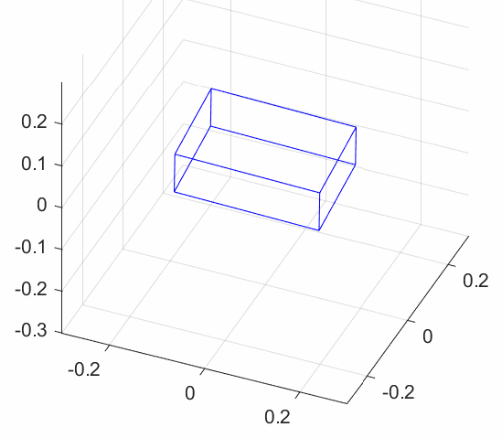
\includegraphics[width=8cm]{./figures/RBRNum1.png}
\caption{动画截图} \label{RBRNum_fig1}
\end{figure}

为了验证数值解的正确性, 我们在生成动画之前用 \lstinline|verify| 函数验证角动量定理, 也就是把力矩函数 \lstinline|tau(t)| 做数值积分, 再与数值解中的角动量进行对比, 结果如\autoref{RBRNum_fig2}.
\begin{figure}[ht]
\centering
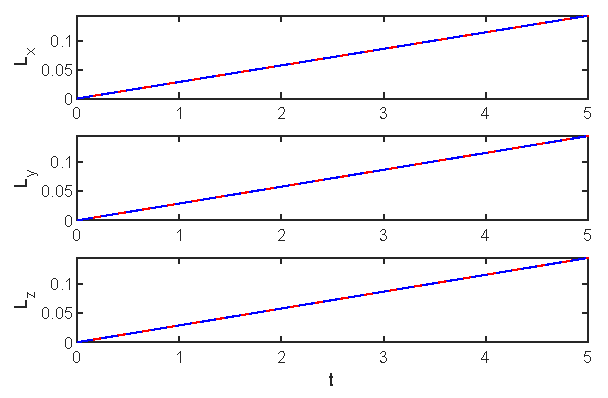
\includegraphics[width=12cm]{./figures/RBRNum1.pdf}
\caption{验证角动量定理, 三个图分别是角动量的三个分量, 蓝线是力矩积分, 红色是数值解中计算的角动量} \label{RBRNum_fig2}
\end{figure}

\Code{rigBdRot}
